\documentclass[12px, a4paper]{article}
\usepackage[utf8]{inputenc}
% ~~~~~~~~~~~~~~~~~~~~~~~~~~~~~~~~~~~~~~~~~~~~~~~~~~~~~~~~~~~~~~~~~~~~~~~~~~~~~~
% Packages to be loaded before others
% ~~~~~~~~~~~~~~~~~~~~~~~~~~~~~~~~~~~~~~~~~~~~~~~~~~~~~~~~~~~~~~~~~~~~~~~~~~~~~~
%%% Packages for LaTeX - programming
%
% Define commands that don't eat spaces.
\usepackage{xspace}
% IfThenElse
\usepackage{ifthen}
%%% Doc: ftp://tug.ctan.org/pub/tex-archive/macros/latex/contrib/oberdiek/ifpdf.sty
% command for testing for pdf-creation
\usepackage{ifpdf} %\ifpdf \else \fi

%%% Internal Commands: ----------------------------------------------
\makeatletter
%
\providecommand{\IfPackageLoaded}[2]{\@ifpackageloaded{#1}{#2}{}}
\providecommand{\IfPackageNotLoaded}[2]{\@ifpackageloaded{#1}{}{#2}}
\providecommand{\IfElsePackageLoaded}[3]{\@ifpackageloaded{#1}{#2}{#3}}

\providecommand{\IfDefined}[2]{%
    \ifcsname #1\endcsname
    #2 %
    \else
    % do nothing
    \fi
}

\providecommand{\IfElseDefined}[3]{%
    \ifcsname #1\endcsname
    #2 %
    \else
    #3 %
    \fi
}
% Calculation with LaTeX
\usepackage{calc}
% Language setting
\usepackage[ngerman]{babel}
% Colors
\usepackage{xcolor}
% Graphics
\usepackage{graphicx}



% ~~~~~~~~~~~~~~~~~~~~~~~~~~~~~~~~~~~~~~~~~~~~~~~~~~~~~~~~~~~~~~~~~~~~~~~~~~~~~~
% Fonts
% ~~~~~~~~~~~~~~~~~~~~~~~~~~~~~~~~~~~~~~~~~~~~~~~~~~~~~~~~~~~~~~~~~~~~~~~~~~~~~~
\usepackage[T1]{fontenc}
% Additional Symbols (Text Companion font extension)
\usepackage{textcomp}



% ~~~~~~~~~~~~~~~~~~~~~~~~~~~~~~~~~~~~~~~~~~~~~~~~~~~~~~~~~~~~~~~~~~~~~~~~~~~~~~
% Math
% ~~~~~~~~~~~~~~~~~~~~~~~~~~~~~~~~~~~~~~~~~~~~~~~~~~~~~~~~~~~~~~~~~~~~~~~~~~~~~~
\usepackage{amsmath}



% ~~~~~~~~~~~~~~~~~~~~~~~~~~~~~~~~~~~~~~~~~~~~~~~~~~~~~~~~~~~~~~~~~~~~~~~~~~~~~~
% Symbols
% ~~~~~~~~~~~~~~~~~~~~~~~~~~~~~~~~~~~~~~~~~~~~~~~~~~~~~~~~~~~~~~~~~~~~~~~~~~~~~~
%%% for Math
%\usepackage{mathrsfs} %% Schreibschriftbuchstaben für den Mathematiksatz (nur Großbuchstaben)
%\usepackage{dsfont}   %% Double Stroke Fonts
%\usepackage[mathcal]{euscript} %% adds euler mathcal font
\usepackage{amssymb}
%\usepackage[Symbolsmallscale]{upgreek} % upright symbols from euler package [Euler] or Adobe Symbols [Symbol]
%\usepackage[upmu]{gensymb}             % Option upmu
%%% common
%\usepackage{wasysym}  %% Doc: http://www.ctan.org/tex-archive/macros/latex/contrib/wasysym/wasysym.pdf
%\usepackage{marvosym} %% Symbols from marvosym Font
%\usepackage{pifont}   %% ZapfDingbats



% ~~~~~~~~~~~~~~~~~~~~~~~~~~~~~~~~~~~~~~~~~~~~~~~~~~~~~~~~~~~~~~~~~~~~~~~~~~~~~~
% Text
% ~~~~~~~~~~~~~~~~~~~~~~~~~~~~~~~~~~~~~~~~~~~~~~~~~~~~~~~~~~~~~~~~~~~~~~~~~~~~~~
%%% Refs
\usepackage[ngerman]{varioref}
\usepackage{hyperref}
%%% Columns
\usepackage{multicol}



% ~~~~~~~~~~~~~~~~~~~~~~~~~~~~~~~~~~~~~~~~~~~~~~~~~~~~~~~~~~~~~~~~~~~~~~~~~~~~~~
% Graphics
% ~~~~~~~~~~~~~~~~~~~~~~~~~~~~~~~~~~~~~~~~~~~~~~~~~~~~~~~~~~~~~~~~~~~~~~~~~~~~~~
\usepackage[all]{xy}
\usepackage{float}
\usepackage{tikz}
%%% Doc: ftp://tug.ctan.org/pub/tex-archive/macros/latex/contrib/subfig/subfig.pdf
% Incompatible: loads package capt-of. Loading of 'capt-of' afterwards will fail therefor
\usepackage{subfig}



% ~~~~~~~~~~~~~~~~~~~~~~~~~~~~~~~~~~~~~~~~~~~~~~~~~~~~~~~~~~~~~~~~~~~~~~~~~~~~~~
% Captions & Style
% ~~~~~~~~~~~~~~~~~~~~~~~~~~~~~~~~~~~~~~~~~~~~~~~~~~~~~~~~~~~~~~~~~~~~~~~~~~~~~~
%%% Doc: ftp://tug.ctan.org/pub/tex-archive/macros/latex/contrib/caption/caption.pdf
\usepackage{caption}
% Aussehen der Captions fuer subfigures (subfig-Paket)
\IfPackageLoaded{subfig}{
    \captionsetup[subfloat]{%
        margin = 10pt,
        font = {small,rm},
        labelfont = {small,bf},
        format = plain, % oder 'hang'
        indention = 0em,  % Einruecken der Beschriftung
        labelsep = space, %period, space, quad, newline
        justification = RaggedRight, % justified, centering
        singlelinecheck = true, % false (true=bei einer Zeile immer zentrieren)
        position = bottom, %top
        labelformat = parens % simple, empty % Wie die Bezeichnung gesetzt wird
    }
}



% ~~~~~~~~~~~~~~~~~~~~~~~~~~~~~~~~~~~~~~~~~~~~~~~~~~~~~~~~~~~~~~~~~~~~~~~~~~~~~~
% Misc
% ~~~~~~~~~~~~~~~~~~~~~~~~~~~~~~~~~~~~~~~~~~~~~~~~~~~~~~~~~~~~~~~~~~~~~~~~~~~~~~
% Theorems
\usepackage{amsthm}
\newtheorem{Definition}{Definition}
\newtheorem{Beispiel}{Beispiel}
\newtheorem{Satz}{Satz}
\newtheorem{Bemerkung}{Bemerkung}
\newtheorem{Algorithmus}{Algorithmus}
\newtheorem{Lemma}{Lemma}
% Listings
\usepackage{listings}
\definecolor{Brown}{cmyk}{0,0.81,1,0.60}
\definecolor{OliveGreen}{cmyk}{0.64,0,0.95,0.40}
\definecolor{CadetBlue}{cmyk}{0.62,0.57,0.23,0}
\definecolor{lightlightgray}{gray}{0.9}
\lstset{
    language=C,                             % Code langugage
    basicstyle=\rm\ttfamily,                % Code font, Examples: \footnotesize, \ttfamily
    keywordstyle=\color{OliveGreen},        % Keywords font ('*' = uppercase)
    commentstyle=\color{gray},              % Comments font
    numbers=left,                           % Line nums position
    numberstyle=\tiny,                      % Line-numbers fonts
    stepnumber=1,                           % Step between two line-numbers
    numbersep=5pt,                          % How far are line-numbers from code
    backgroundcolor=\color{lightlightgray}, % Choose background color
    frame=none,                             % A frame around the code
    tabsize=2,                              % Default tab size
    captionpos=b,                           % Caption-position = bottom
    breaklines=true,                        % Automatic line breaking?
    breakatwhitespace=false,                % Automatic breaks only at whitespace?
    showspaces=false,                       % Dont make spaces visible
    showtabs=false,                         % Dont make tabls visible
    %columns=flexible,                       % Column format
    %morekeywords={someword, otherword},     % specific keywords
}

\usepackage{amsmath}
\usepackage{hyperref}
\hypersetup{
    colorlinks=true,     
    urlcolor=blue
}
\usepackage{float}
\usepackage{algorithm}
\usepackage{arevmath}     % For math symbols
\usepackage[noend]{algpseudocode}

\begin{document}
\setlength{\parindent}{0em}
%front
\title{ Stochastik}
\author{Dr. Johannes Riesterer}
\date{\today}
\maketitle\thispagestyle{empty}
 \begin{figure}[H]
    \centering
    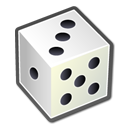
\includegraphics[width=1.0 \textwidth]{images/cover.png}
    \label{fig:diffus}
\end{figure}
\newpage 
\begin{center}
\large
 \copyright Johannes Riesterer \\
\end{center}
\thispagestyle{empty}
\newpage

\section*{Vorwort}
Kann jeder Mathematik lernen? Als Antwort auf diese Frage möchte ich auf den interessanten Lebenslauf
einer der bedeutendsten Mathematikerinnen aller Zeiten eingehen  (Auszug aus Wikipedia):

Emmy Noether war eine deutsche Mathematikerin, die grundlegende Beiträge zur abstrakten Algebra und zur theoretischen Physik lieferte. Insbesondere hat Noether die Theorie der Ringe, Körper und Algebren revolutioniert. Das nach ihr benannte Noether-Theorem gibt die Verbindung zwischen Symmetrien von physikalischen Naturgesetzen und Erhaltungsgrößen an. 

Sie zeigte in mathematischer Richtung keine besondere Frühreife, sondern hatte in ihrer Jugend Interesse an Musik und Tanzen. Sie besuchte die Städtische Höhere Töchterschule – das heutige Marie-Therese-Gymnasium – in der Schillerstraße in Erlangen. Mathematik wurde dort nicht intensiv gelehrt. Im April 1900 legte sie die Staatsprüfung zur Lehrerin der englischen und französischen Sprache an Mädchenschulen in Ansbach ab. 1903 holte sie in Nürnberg die externe Abiturprüfung am Königlichen Realgymnasium – dem heutigen Willstätter-Gymnasium – nach. 


\newpage

%Einfügen des Inhaltsverzeichnisses
\tableofcontents
\newpage
\thispagestyle{empty}
\mbox{}\thispagestyle{empty}
\newpage
%main

\section{Notationen}

Für eine Menge $\Omega$ bezeichnet $\# \Omega$ die Anzahl ihrer Elemente und $\mathcal{P} (\Omega) : = \{ A \, | \, A \subseteq \Omega \}$ die Potenzmenge von $\Omega$. 


\begin{figure}[htp]
      \centering
    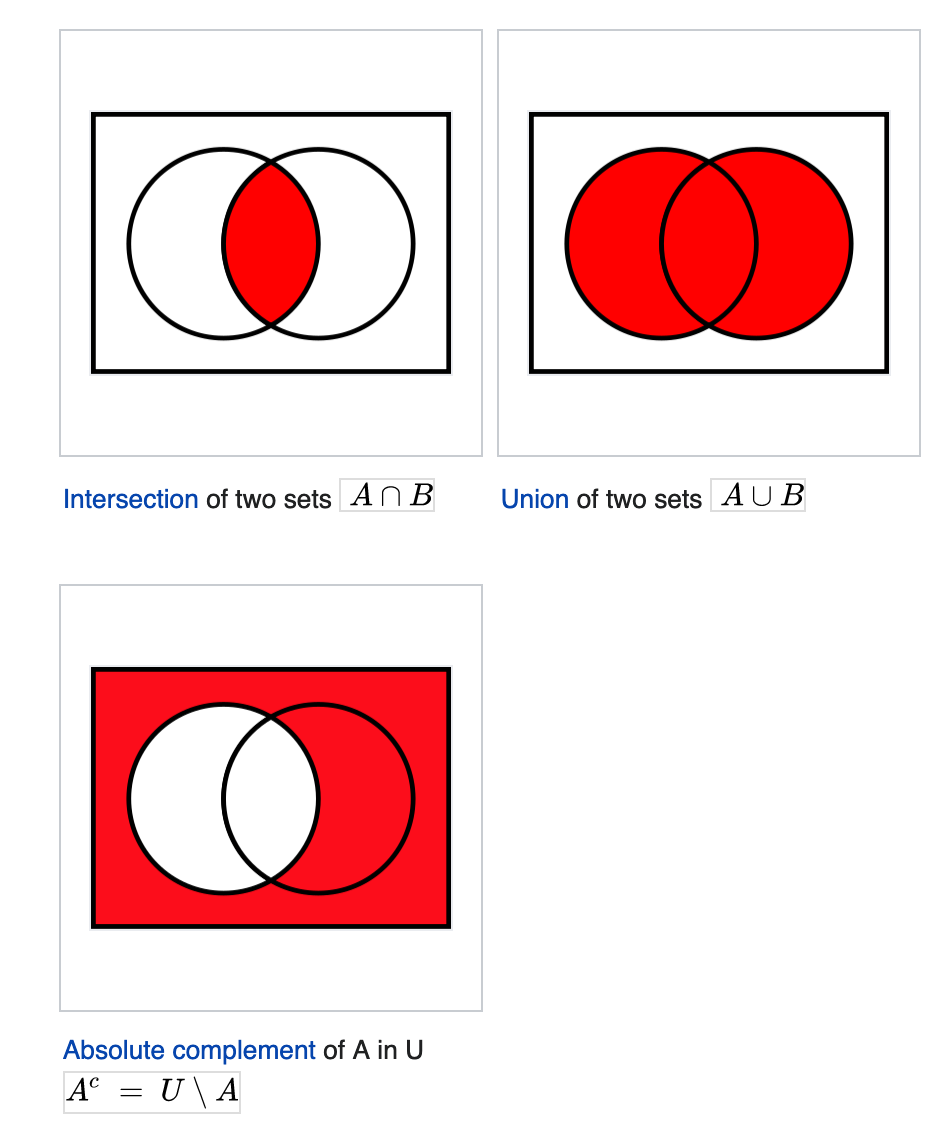
\includegraphics[width=0.9\textwidth]{images/Venn}

      \caption{Quelle: Wikipedia}
\end{figure}


\begin{figure}[htp]
      \centering
    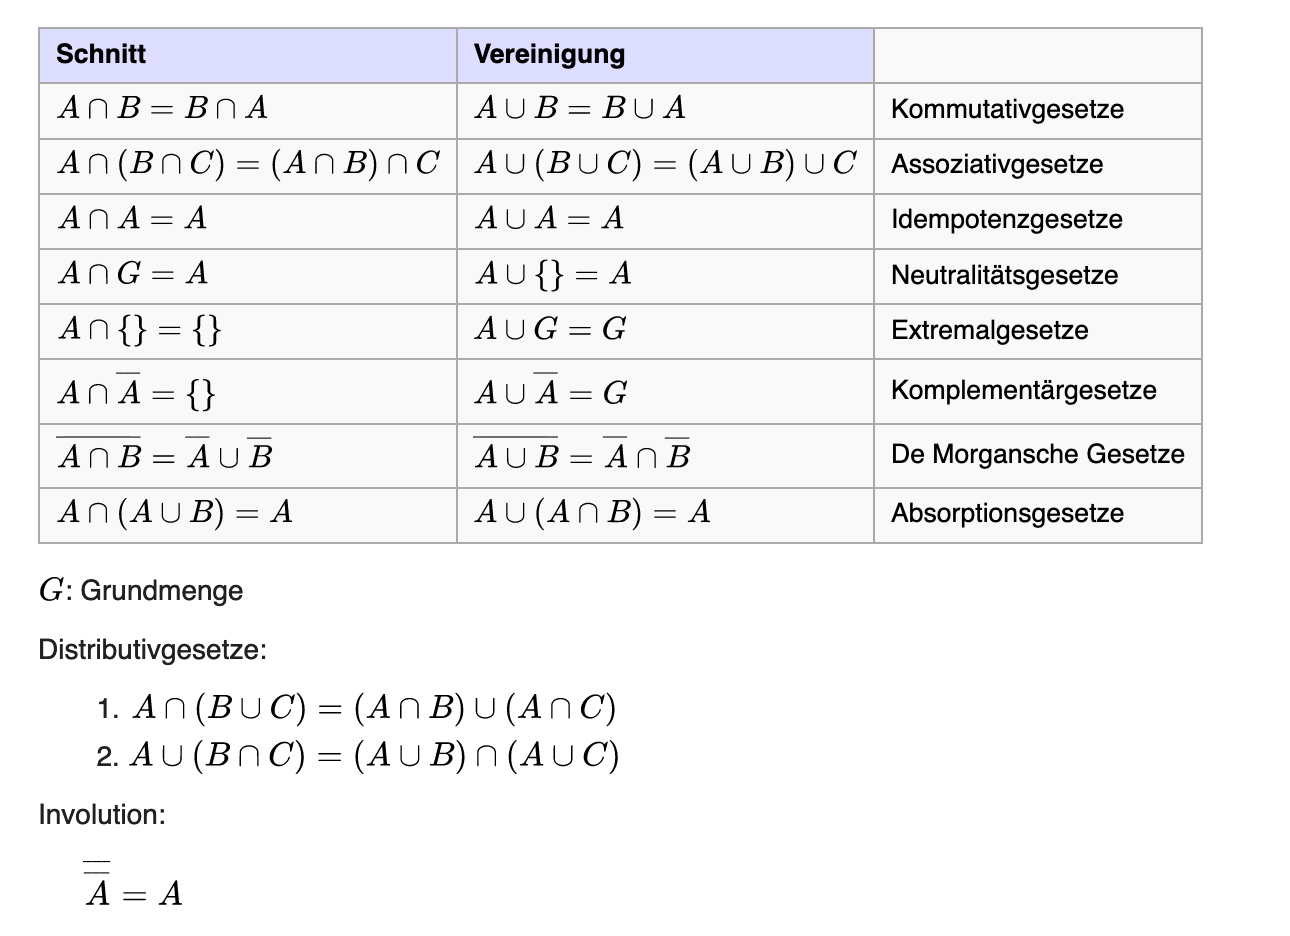
\includegraphics[width=0.9\textwidth]{images/mengengesetze}

      \caption{Quelle: Wikipedia}
\end{figure}



\newpage

\section{Diskrete Modelle}

\begin{Definition}[Laplace Wahrscheinlichkeit]~
Sei $\Omega = \{ \omega_1, \cdots , \omega_n\}$ eine endliche Menge. Für $A \subseteq \Omega$ definieren wir die Wahrscheinlichkeit durch
\begin{align*}
P(A) : = \frac{\#A}{ \# \Omega} \; . 
\end{align*} 
Die Elemente $ \omega_1, \cdots , \omega_n \in \Omega$ nennen wir Elementarereignisse und Teilmengen $A \subseteq \Omega$ Ereignisse. Die Abbildung
\begin{align*}
P : \mathcal{P} (\Omega) \to [0,1]  
\end{align*}  
nennen wir die Laplace-Verteilung bzw. Gleichverteilung auf $\Omega$.
\end{Definition}


\begin{Definition}[Variationen und Kombinationen]~
\begin{itemize}
\item $Var_k^n(\Omega, m.W.) : = \{ ( \omega_1, \ldots, \omega_k) \ |\  \omega_i \in \Omega \}$  Menge aller Variationen mit Wiederholung.
\item $Var_k^n(\Omega, o.W.) : = \{ ( \omega_1, \ldots, \omega_k) \ |\  \omega_i \in \Omega; \;  \omega_i \neq \omega_j  \}$  Menge aller Variationen ohne Wiederholung.
\item $Kom_k^n(\Omega, m.W.) : = \{ ( \omega_{i_1}, \ldots, \omega_{i_k})  \ |\  \omega_{i_l} \in \Omega; \; 1  \leq i_1 \leq  \ldots  \leq i_k  \}$  Menge aller Kombinationen  mit Wiederholung.
\item $Kom_k^n(\Omega, o.W.) : = \{ ( \omega_{i_1}, \ldots, \omega_{i_k} ) \ |\  \omega_{i_l} \in \Omega; \; 1 \leq i_1  \leq \ldots \leq i_k; \;  \omega_{i_i} \neq \omega_{i_j} \} $  Menge aller Kombinationen  ohne  Wiederholung.
\end{itemize}
\end{Definition}

\begin{Lemma}~
\begin{itemize}
\item $\# Var_k^n(\Omega, m.W.)  = n^k = \underbrace{n \cdot n \cdots n}_{\text{k-mal}}$
\item $\# Var_k^n(\Omega, o.W.)  = n_k = n \cdot (n-1) \cdots  (n-(k-1)) = \frac{n!}{(n-k)!}$  
\item $\#Kom_k^n(\Omega, o.W.) = \binom{n}{k} = \frac{n!}{k! (n-k)!}$  
\item $\#Kom_k^n(\Omega, m.W.)  = \binom{n + k -1}{k}$  
\end{itemize}
\end{Lemma}

\begin{Definition}[Diskrete Wahrscheinlichkeitsverteilung]~
Es sei $\Omega$ eine (nicht leere) abzählbare Menge. Eine Abbildung 
$P :\mathcal{P}(\Omega) \to [0,1]$ heißt diskrete Wahrscheinlichkeitsverteilung (Wahrscheinlichkeitsmaß), falls gilt:
\begin{align*}
& P(\Omega) = 1\\
& P \Biggl( \bigcup_{n=1}^{\infty} A_n \biggr)= \sum_{n=1}^{\infty} P(A_n), \text{ mit } A_i \cap A_j = \emptyset \text{ für } i \neq j 
\end{align*}
\end{Definition}


\begin{Beispiel}[Laplace Wahrscheinlichkeit]~
$\Omega$ endlich und $P(A) = \frac{\#A}{\#\Omega}$.
 \end{Beispiel}


\begin{Definition}[Bedingte  Wahrscheinlichkeit]~
Für $A,B \in \mathcal{A}$ und $P(B) > 0$ heißt
\begin{align*}
& P(A \; | \;  B) = \frac{P(A \cap B)}{P(B)} \\
\end{align*}
die bedingte Wahrscheinlichkeit (von $A$ unter $B$).
\end{Definition}


\begin{figure}[htp]
      \centering
    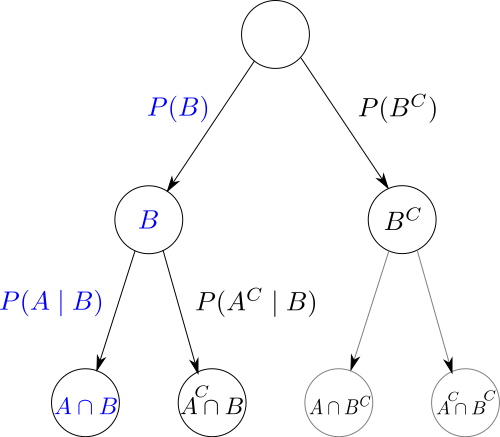
\includegraphics[width=0.5\textwidth]{images/Probability_tree}

      \caption{Quelle: Wikipedia}
\end{figure}



\begin{Satz}[Satz der totalen Wahrscheinlichkeit]
Für eine Zerlegung  $\Omega = \bigcup_{j=1}^{n} B_j, \text{ mit } B_i \cap B_k = \emptyset \text{ für } i \neq k $
\begin{align*}
& P(A ) = \sum_{j=1}^{n}  P(A \; | \;  B_j) \cdot P(B_j)
\end{align*}
\end{Satz}
\begin{proof}
$A = A \cap B \cup A \cap \bar{B}$ und  $A \cap B \cap A \cap \bar{B} = \emptyset$. 
\begin{align*}
& P(A) =  P(A \cap B) + P(A \cap \bar{B}) = P(B) \cdot P(A  \; | \; B) + P(\bar{B}) \cdot P(A  \; | \; \bar{B}) 
\end{align*}
\end{proof}

\begin{Satz}[Satz von Bayes]
Für $A,B \in  \mathcal{A}$ mit  $P(B) > 0$ gilt
\begin{align*}
& P(A \; | \;  B) = \frac{P(B \; | \; A) \cdot P(A)} {P(B)} \\
\end{align*}
\end{Satz}

\begin{proof}
\begin{align*}
& P(A \; | \;  B) =\frac{P(A \cap B)}{P(B)} = \frac{ \frac{P(A \cap B) \cdot P(A)}{P(A)}}{P(B)}  =  \frac{P(B \; | \; A) \cdot P(A)} {P(B)} 
\end{align*}
\end{proof}


\begin{Definition}[Stochastische Unabhängigkeit]
Zwei Ereignisse $A,B$ heißen stochastisch unabhängig, falls
\begin{align*}
P(A \cap B) = P(A) \cdot P(B)
\end{align*}
gilt.  Somit ist auch $P(A | B) = P(A)$ und $P(B  | A) = P(B)$.
\end{Definition}


\subsection{Naiver Bayes'scher Spam Filter}
Gegeben ist eine E-Mail $E$.  Wir möchten anhand des Vorkommens bestimmter Wörter $A_1, \ldots A_n$ in der Mail entscheiden, ob es sich um eine erwünschte Mail $H$ oder eine unerwünschte Mail $S$ (Ham or Spam) handelt. 
(Typische Wörter wären zum Beispiel "reichwerden",  "onlinecasino" ...)
Aus einer Datenbank kann man das Vorkommen dieser Wörter in Spam und Ham Mails zählen und damit empirisch die Wahrscheinlichkeiten $P(A_i | S)$ und $P(A_i | H) $ des Vorkommens dieser Wörter in Spam und Ham Mails ermitteln.  Wir gehen davon aus, dass es sich bei der Mail  prinzipiell mit  Wahrscheinlichkeit $P(E= S) = P(E= H)= \frac{1}{2}$  um eine erwünschte  Mail $H$ oder eine unerwünschte Mail $S$  handeln kann. 




 Wir machen zudem die (naive) Annahme, dass das Vorkommen der Wörter  stochastisch unabhängig ist, also 
\begin{align*}
P(A_1 \cap \cdots \cap A_n | S) = P(A_1 | S) \cdots P(A_n | S) \\
P(A_1 \cap \cdots \cap A_n | H) = P(A_1 | H) \cdots P(A_n | H)
\end{align*}
gilt.


Mit der Formel von Bayes und der totalen Wahrscheinlichkeit  können wir somit berechnen
\begin{align*}
& P(E=S |  A_1 \cap \cdots \cap A_n) = \frac{P(A_1 \cap \cdots \cap A_n | S) \cdot P(S)}{P(A_1 \cap \cdots \cap A_n)} \\
&=  \frac{P(A_1 | S) \cdots P(A_n | S) \cdot P(S)}{P(A_1 \cap \cdots \cap A_n | H) + P(A_1 \cap \cdots \cap A_n | S)} \\
&=  \frac{P(A_1 | S) \cdots P(A_n | S) \cdot P(S)}{P(A_1 | H) \cdots P(A_n | H)  + P(A_1 | S) \cdots P(A_n | S) } \\
\end{align*}
Bemerkung: $P(E=H |  A_1 \cap \cdots \cap A_n) = 1- P(E=S |  A_1 \cap \cdots \cap A_n) $


\section{Zufallsvariablen}

\begin{Definition}
Ein Messraum ist ein Paar $(\Omega, \mathcal{A})$ bestehend aus einer Menge $\Omega$ und einer Sigma-Algebra $\mathcal{A} \subset \mathcal{P}(\Omega)$.
\end{Definition}



\begin{Definition}
Sei $(\Omega, \mathcal{A}, P)$ ein Wahrscheinlichkeitsraum und $(\Omega', \mathcal{A}')$ ein Messraum. Eine Zufallsvariable ist eine Abbildung
$$X : \Omega \to \Omega'$$ 
so dass für alle Ereignisse $A' \in  \mathcal{A}'$
$$ X^{-1} (A') \in \mathcal{A}$$
 ein Ereignis in $\mathcal{A}$ ist. Urbilder von Ereignissen sind also Ereignisse.
\end{Definition}

\begin{Definition}
Sei $(\Omega, \mathcal{A}, P)$ ein Wahrscheinlichkeitsraum, $(\Omega', \mathcal{A}')$ ein Messraum und  $X : \Omega \to \Omega'$  Eine Zufallsvariable. 
Durch 
\begin{align*}
P_X (A') := P(X^{-1} (A'))
\end{align*}
 für $A' \in \mathcal{A}'$ wird ein Wahrscheinlichkeitsmaß auf  $(\Omega', \mathcal{A}')$ definiert. Es wird Bildmaß genannt. Anstelle von $P_X (A')$ wird auch die Schreibweise $P (X \in A'):= P_X (A')$ verwendet.
\end{Definition}

\begin{Definition}
Sei $(\Omega, \mathcal{A}, P)$ ein Wahrscheinlichkeitsraum, $(R, \mathcal{B})$ ein Messraum  und
 $\{X_i\}_{i=1}^n$ ein Folge von Zufallsvariablen   $X_i :  \Omega \to R$.
Die zufallsvariablen heissen identisch verteilt, falls
 $P_{X_i} = P_{X_j}$ für alle $i,j$  und
stochastisch unabhängig, falls
 $P_{(X_1, \cdots ,X_n)} = \prod_{i=1}^n P_{X_i}$ gilt. 
\end{Definition}


\subsection{Integration bezüglich eines Wahrscheinlichkeitsmaßes}
in diesem Abschnitt ist  $(\Omega, \mathcal{A},P)$ ein fest gewählter Wahrscheinlichkeitsraum.

\begin{Definition}
Für eine Teilmenge $A \in \mathcal{A}$ heißt
$$ 1_A (x): = \begin{cases} 1 \text{  falls }   x \in A  \\  0  \text{  sonst}  \end{cases}$$
Indikatorfunktion.
\end{Definition}

\begin{Definition}
Eine Funktion 
$$ \varphi(x) := \sum_{k=1}^m c_k 1_{A_k}(x)$$ mit $c_k \in \mathbb{R}$ und $A_k \in \mathcal{A}$ mit $A_i \cap A_j = \emptyset$ für $i \neq j$
heißt Treppenfunktion.
\end{Definition}





\begin{Definition}
Eine Hüllreihe zu einer Funktion $f :\Omega \to \mathbb{R}$ ist eine Reihe $\phi(x):= \sum_{k=1}^{\infty} c_k  1_{A_k} (x)$ mit den folgenden Eigenschaften:
\begin{itemize}
\item $c_k \in \mathbb{R}$ sind positive reelle Zahlen $c_k >0$.
\item $A_k \in \mathcal{A}$.
\item Für alle $x \in \Omega$ gilt $|f(x) | \leq \phi(x)$.
\end{itemize}
\end{Definition}

 
\begin{Definition}
Für eine Treppenfunktion $ \varphi(x) := \sum_{k=1}^m c_k 1_{A_k}(x)$ definieren wir das Integral durch
$$\int_{\Omega} \varphi dP := \sum_{k =1}^m  c_k P(A_k) \; . $$
\end{Definition}


\begin{Definition}
Der Inhalt einer Hüllreihe $\phi(x):= \sum_{k=1}^{\infty} c_k  1_{A_k} (x)$ ist definiert durch 
$$I_P (\phi) := \sum_{k=1}^{\infty} c_k \;  P(A_k) \; .$$
\end{Definition}


\begin{Definition}
Die $L_{P^1}$-Halbnorm einer Funktion $f : \Omega\to \mathbb{R}$ ist definiert durch das Infimum der Inhalte der Hüllreihen zu $f$
$$ || f ||_{P^1} : = \inf  \biggl \{   I(\phi) \; | \; \phi  \text{ ist Hüllreihe zu  }  f \biggr \} \; .$$
\end{Definition}



\begin{Definition}
Eine Funktion $f : \Omega \to \mathbb{R}$ heißt integrierbar, falls eine Folge von Treppenfunktionen  $\varphi_k$ existiert mit
$$ || f -  \varphi_k ||_{P^1} \to 0 \text{ für } k \to \infty \;. $$
In diesem Fall heißt
$$ \int_{\Omega} f(x) dP := \lim_{k \to \infty}  \int_{\Omega}  \varphi_k  dP$$
das Integral von $f$ über $\Omega$.
\end{Definition}


\subsection{Reelle Zufallsvariablen}

\begin{Definition}
Eine Menge $U \subset  \mathbb{R}^n$ heißt offen, falls für jeden Punkt $x \in U$ ein Radius $\epsilon > 0$ existiert, so dass der Ball $B_\epsilon (x)$ in $U$ enthalten ist, also 
$B_\epsilon (x) \subset U$ gilt.
\end{Definition}

\begin{figure}[htp]
      \centering
    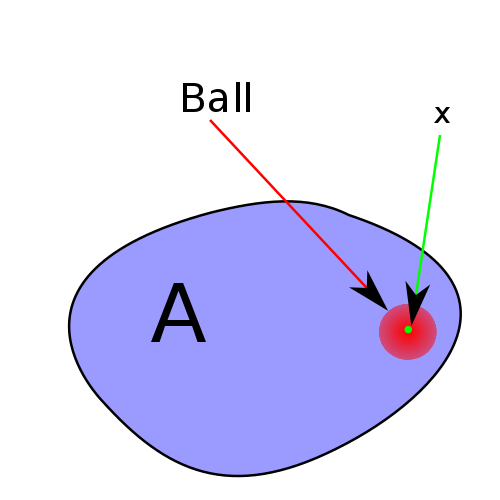
\includegraphics[width=0.45\textwidth]{images/openset}
      \caption{Quelle: Wikipedia}
\end{figure}


\begin{Definition}
Die Borel'sche   $\sigma$-Algebra $\mathcal{B}(\mathbb{R}^n)$über $\mathbb{R}^n$ ist die kleinste  $\sigma$-Algebra, die alle offenen Mengen $\mathcal{U}$ enthält, also 
\begin{align*}
A_\sigma (\mathcal{U}) := \bigcap \{  \mathcal{A} \subset \mathcal{P}(\mathbb{R}^n);  \;   \mathcal{U}  \subset  \mathcal{A},  \;  \mathcal{A} \text{ ist $\sigma$-Algebra} \}
\end{align*}
\end{Definition}

\begin{Satz}
Die Borel'sche   $\sigma$-Algebra existiert, da die Potenzmenge eine   $\sigma$-Algebra ist.
\end{Satz}

\begin{Satz}
Die Borel'sche   $\sigma$-Algebra ist in der $\sigma$-Algebra der Lebesgue messbaren Mengen enthalten.
\end{Satz}

\begin{Definition}
Unter einer reellen Zufallsvariable verstehen wir eine Zufallsvariable 
\begin{align*}
& X : \Omega \to \mathbb{R}^n \\
& X(\omega) := \biggl(X_1(\omega), \cdots , X_n(\omega)  \biggr) \; ,
\end{align*}
wobei $(\Omega, \mathcal{A}, P)$ ein Wahrscheinlichkeitsraum ist und $(\mathbb{R}^n, \mathcal{B}(\mathbb{R}^n)$ der $\mathbb{R}^n$ zusammen mit der Borell'schen Sigma-Algebra ist. Das Integral ist komponentenweise definiert durch
\begin{align*} 
\int_{\Omega} X dP :=  \biggl( \int_{\Omega} X_1 dP, \cdots , \int_{\Omega} X_n dP    \biggr)
\end{align*}

\end{Definition}



\subsection{Erwartungswert}
\begin{Satz}
Eine reelle Zufallsvariable ist integrierbar.
\end{Satz}

\begin{Definition}
Für eine reelle Zufallsvariable heißt 
\begin{align*} 
& F_X : \Omega \to [0,1] \\
& F_X (x) := P (X \leq x) := P_X (( -\infty, x ) = P(X^{-1} (-\infty, x))
\end{align*}
Verteilungsfunktion von $X$.
\end{Definition}




\begin{Definition}
Sei $\Omega \subset \mathbb{R}^n$ und $(\Omega, \mathcal{A})$ ein Messraum wobei alle $A \in \mathcal{A}$ Lebebesgue-messbar sind.
 Eine Funktion $f: \Omega \to \mathbb{R}$ heiß Dichte, falls für ihr Lebesgue-Integral $\int_{\Omega} f d \mu = 1$ gilt.
\end{Definition}

\begin{Beispiel}
Die Funktion $f(x) = \frac{1}{\sqrt{\pi}} e^{- x^2}$ ist eine Dichte auf $ \mathbb{R}$.
\begin{align*}
& I := \int_{0}^{\infty} e^{-x^2} \; dx\\
& I^2 = \int_{0}^{\infty} \int_{0}^{\infty} e^{-(x^2+y^2)} \; dx \;dy \\
&x=r \cos \varphi ,y=r\sin \varphi ,r^2 = x^2 + y^2  \; (\text{ da } \cos^2 + \sin^2 = 1)\\
 &\text{ \href{https://de.wikipedia.org/wiki/Polarkoordinaten\#Zylinderkoordinaten}{LINK: Polarkoordinatentransformation}} \\
& = \int_{0}^{\frac{\pi}{2}}  \int_{0}^{\infty}r \cdot e^{-r^2} \; dr \;d\varphi \\
&= \frac{\pi}{2} \int_{0}^{\infty}r \cdot e^{-r^2} \; dr \\
&= -\frac{\pi}{4} [e^{-r^2} ]_0^{\infty} = \frac{\pi}{4} \Rightarrow I = \frac{\sqrt{\pi}}{2}
\end{align*}
Analog beweist man, dass für alle  $\mu \in \mathbb{R}, \sigma > 0 $ die Funktion $ f(x):=  \frac 1{\sigma \sqrt{2\pi}}e^{- \frac {1}{2} (\frac{x- \mu}{ \sigma})^2}dx$  eine  Dichte auf $ \mathbb{R}$ ist.
\end{Beispiel}

\begin{figure}[htp]
      \centering
    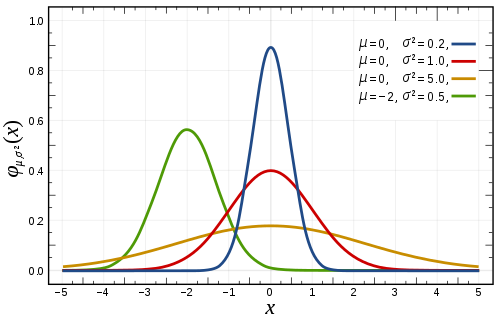
\includegraphics[width=0.96\textwidth]{images/normal}
      \caption{Quelle: Wikipedia}
\end{figure}


\begin{Definition}[Normalverteilung]
Eine reelle Zufallsvariable $X: \Omega \to \mathbb{R}$ heisst Normalverteilt, wenn 
$F_X (x) = \int_{- \infty}^{x}  \frac 1{\sigma \sqrt{2\pi}}e^{- \frac {1}{2} (\frac{x- \mu}{ \sigma})^2}dx$ mit  $\mu \in \mathbb{R}, \sigma > 0 $gilt. Man schreibt auch $X \sim \mathcal{N}(\mu, \sigma^2)$.
\end{Definition}
\begin{figure}[htp]
      \centering
    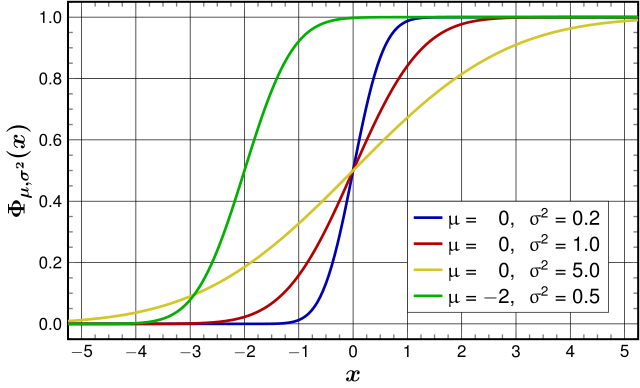
\includegraphics[width=0.96\textwidth]{images/normal_distribution}
      \caption{Quelle: Wikipedia}
\end{figure}


\subsection{Erwartungswert}


\begin{Definition}
Für eine reelle Zufallsvariable ist der Erwartungswert definiert durch
$$ \mathbb{E} (X) := \int_{\Omega} X dP \; .$$
\end{Definition}




\begin{Bemerkung}
Ist $(\Omega, \mathcal{A}, P)$ ein diskreter Wahrscheinlichkeitsraum und $X :\Omega \to \mathbb{R}$ eine eindimensionale reelle Zufallsvariable, so ist
$$ \mathbb{E} (X) = \sum_{\omega \in \Omega}  X(\omega) \cdot P(\omega)$$
\end{Bemerkung}


\begin{Satz}
Für eine reelle Zufallsvariable $X: \Omega \to \mathbb{R}^n$ und eine integrierbare Funktion $g:  \mathbb{R}^n \to \mathbb{R}$ gilt
$$ \mathbb{E} (g \circ X) := \int_{\Omega} g \circ X dP = \int_{\mathbb{R}^n}  g  dP_X \;. $$
Ist insbesondere $f(x) : \mathbb{R}^n \to \mathbb{R}$ eine Dichte für $P_X$ , so ist  
$$\mathbb{E} (X) =  \int_{\mathbb{R}^n} x \cdot f(x) d\mu$$ das Lebesgue-Integral der Funktion $x \cdot f(x)$.

\end{Satz}

\begin{proof}
Für $g = 1_A$ mit $A \in \mathcal{B}(\mathbb{R}^n)$ ist
\begin{align*}
& \int 1_A dP_X = P_X(A) = P(X^{-1} (A)) = \int 1_{X^{-1}(A)} dP \\
&= \int 1_{A} \circ X dP
\end{align*}
Für eine Treppenfunktion $g= \sum_{i= 1}^n c_i 1_{A_i} $folgt das Ergebnis aus der Linearität des Integrals für Treppenfunktionen. Für integrierbares $g$ folgt das Resultat mit Hilfe von Konvergenzsätzen für das  Integral.
\end{proof}



\begin{Beispiel}
$\Omega = \{ \text{Kopf},\text{Zahl}\}$, $P(\text{Kopf}) = P(\text{Zahl}) = \frac{1}{2}$, $X(\text{Kopf}) = 0,  X(\text{Zahl}) = 1$ 
\begin{align*}
& \mathbb{E}(X)  = 0 \cdot P(X^{-1}(0) ) + 1 \cdot P(X^{-1}(1)) \\
& =0  \cdot P(\text{Kopf}) + 1 \cdot P(\text{Zahl}) = \frac{1}{2}  
\end{align*}
\end{Beispiel}

\begin{Beispiel}
Sei $X \sim \mathcal{N}(\mu, \sigma^2)$.
\begin{align*}
\mathbb{E}(X) & := \int_{\mathbb{R}}  x \cdot  \frac 1{\sigma \sqrt{2\pi}}e^{- \frac {1}{2 } (\frac{x- \mu}{ \sigma})^2} \; dx  \\
&= \int_{\mathbb{R}}  (y + \mu) \cdot  \frac 1{\sigma \sqrt{2\pi}}e^{- \frac {1}{2 \sigma^2} y^2} \; dy \\
 &  = \mu  \int_{\mathbb{R}}      \frac 1{\sigma \sqrt{2\pi}}e^{- \frac {1}{2 \sigma^2} y^2} \; dy  + \int_{\mathbb{R}}  y  \cdot  \frac 1{\sigma \sqrt{2\pi}}e^{- \frac {1}{2 \sigma^2} y^2} \; dy = \mu
\end{align*}
\end{Beispiel}

\begin{Satz}
Sind $X,Y : \Omega \to \mathbb{R}^n$   reelle, integrierbare  Zufallsvariablen und $a,b \in \mathbb{R}$ konstant, so gilt:
\begin{align*}
& \mathbb{E}(a \cdot X + b \cdot Y) = a \cdot \mathbb{E}(X) + b \cdot \mathbb{E}(Y) \\
& X(x) \leq Y(x) \;  \forall x \in \Omega \Rightarrow \mathbb{E}(X) \leq \mathbb{E}(Y) \\
& X ,Y \text{ stoch. unabhängig} \Rightarrow   \mathbb{E}(X \cdot Y) =  \mathbb{E}(X) \cdot  \mathbb{E}(Y) \\
& \mathbb{E} (1_A) = P (A)
\end{align*}
\end{Satz}

\begin{Satz}{Markov-Ungleichung }
Sei $Y : \Omega \to \mathbb{R}$  eine  reelle, integrierbare  Zufallsvariablen und $f : [0, \infty) \to [0, \infty)$ monoton wachsend.
Dann gilt für alle $\epsilon > 0$ mit $f(\epsilon) > 0$
\begin{align*}
P (|Y |  \geq \epsilon) \leq \frac{\mathbb{E} (f \circ |Y|)}{f(\epsilon)}
\end{align*}
\end{Satz}
\begin{proof}
Da $f(\epsilon) 1_{\{ |Y| \geq  \epsilon \} } \leq f \circ |Y|$ folgt
\begin{align*}
f(\epsilon) P(|Y| \geq \epsilon) = & f(\epsilon) \mathbb{E}(1_{\{ |Y| \geq  \epsilon \} }) = \mathbb{E}( f(\epsilon) 1_{\{ |Y| \geq  \epsilon \} }) \\
\leq & \mathbb{E}( f \circ |Y|)
\end{align*}
\end{proof}


\subsection{Varianz}

\begin{Definition}
Für eine reelle Zufallsvariable ist die Varianz definiert durch
$$ \mathbb{V} (X) :=  \mathbb{E}( (X - \mathbb{E}(X)^2)) \; .$$
\end{Definition}

\begin{Satz}{Verschiebungssatz}
\begin{align*}
 \mathbb{V}(X) & = \mathbb{E}(X^2 - 2X \mathbb{E}(X) + \mathbb{E}(X)^2) = \mathbb{E}(X^2) - 2 \mathbb{E}(X)^2 +  \mathbb{E}(X)^2 \\
& =  \mathbb{E}(X^2) -  \mathbb{E}(X)^2 \\
\end{align*}
\end{Satz}

\begin{Beispiel}
Sei $X \sim \mathcal{N}(\mu, \sigma^2)$.
\begin{align*}
&\mathbb{V} (X) =  \frac{1}{\sqrt{2 \pi}} \int_{- \infty}^{\infty} x^2 e^{- \frac{x^2}{2}} \; dx =   \frac{1}{\sqrt{2 \pi}} \int_{- \infty}^{\infty} x (xe^{- \frac{x^2}{2}}) \; dx \\
& =  \frac{1}{\sqrt{2 \pi}} \biggl (\biggl [ x (e^{- \frac{x^2}{2}}) \biggr]_{- \infty}^{\infty}   - \int_{- \infty}^{\infty}  - e^{- \frac{x^2}{2}} \; dx  \biggr) = 0 + 1 = 1\\
\end{align*}
\href{https://de.wikipedia.org/wiki/Partielle_Integration}{LINK: Partielle Integration}. Mit "Verschiebungstrick"
$\Rightarrow \mathbb{V}(X) = \sigma^2$.
\end{Beispiel}




\begin{Satz}{Tschebyscheff-Ungleichung }
Für eine  eine  reelle, integrierbare und quadratintegrierbare  Zufallsvariablen $Y : \Omega \to \mathbb{R}$  gilt:
\begin{align*}
P (|Y  - \mathbb{E} (Y)|  \geq \epsilon) \leq \frac{\mathbb{V} (Y)}{ \epsilon^2} 
\end{align*}
\end{Satz}
\begin{proof}
Folgt direkt aus der Markov-Ungleichung mit $Y' = Y -\mathbb{E}(Y)$ und $f(x) = x^2$
\end{proof}



\begin{Satz}{Schwaches Gesetzt der großen Zahlen }
Seien $X_i : \Omega \to \mathbb{R}$ unabhängige, reelle Zufallsvariablen (uid, iid(englisch)) mit $\mathbb{E}(X_i) = \mu < \infty$ und $\mathbb{V}(X_i) = \sigma < \infty$, dann gilt
\begin{align*}
P \bigl  ( \bigl | \frac{1}{n} \sum_{i=1}^{n} X_i - \mu \bigr |  \geq \epsilon \bigr) \leq \frac{\sigma}{ n \cdot \epsilon^2} \; \; \underset{n \to \infty}{\longrightarrow} 0
\end{align*}
(stochastische Konvergenz). 
\end{Satz}
\begin{proof}
Mit $Y_n =  \frac{1}{n} \sum_{i=1}^{n}  X_i - \mu$ ist $\mathbb{E}(Y_n) =  \frac{1}{n} \sum_{i=1}^{n} \mathbb{E}( X_i - \mu) = 0$ und 
$\mathbb{V}(Y_n) =  \frac{1}{n^2} \sum_{i=1}^{n} \mathbb{V}( X_i ) = \frac{\sigma}{n}$. Aus der Tschebyscheff-Ungleichung folgt die Behauptung.
\end{proof}





%back
\newpage
\listoftables{\addcontentsline{toc}{section}{\listtablename}}
\newpage
\listoffigures{\addcontentsline{toc}{section}{\listfigurename}}
\newpage
\IfDefined{printindex}{\printindex}
\IfDefined{printnomenclature}{\printnomenclature[4.5cm]{}}
\end{document}
